

%----------------------------------------------------------------------------------------
%	PACKAGES AND OTHER DOCUMENT CONFIGURATIONS
%----------------------------------------------------------------------------------------

\documentclass{article}

\usepackage{fancyhdr} % Required for custom headers
\usepackage{lastpage} % Required to determine the last page for the footer
\usepackage{extramarks} % Required for headers and footers
\usepackage[usenames,dvipsnames]{color} % Required for custom colors
\usepackage{graphicx} % Required to insert images
\usepackage{listings} % Required for insertion of code
\usepackage{courier} % Required for the courier font
\usepackage{algorithm}

\usepackage{algpseudocode} 

% Margins
\topmargin=-0.45in
\evensidemargin=0in
\oddsidemargin=0in
\textwidth=6.5in
\textheight=9.0in
\headsep=0.25in

\linespread{1.1} % Line spacing

% Set up the header and footer
\pagestyle{fancy}
\lhead{\hmwkAuthorName\ : \hmwkStudentID} % Top left header
%\chead{ \hmwkClassShort} % Top center head
\rhead{\firstxmark} % Top right header
\lfoot{\lastxmark} % Bottom left footer
\cfoot{} % Bottom center footer
\rfoot{Page\ \thepage\ of\ \protect\pageref{LastPage}} % Bottom right footer
\renewcommand\headrulewidth{0.4pt} % Size of the header rule
\renewcommand\footrulewidth{0.4pt} % Size of the footer rule

\setlength\parindent{0pt} % Removes all indentation from paragraphs

%----------------------------------------------------------------------------------------
%	CODE INCLUSION CONFIGURATION
%----------------------------------------------------------------------------------------

\definecolor{MyDarkGreen}{rgb}{0.0,0.4,0.0} % This is the color used for comments
\lstloadlanguages{C} % Load Perl syntax for listings, for a list of other languages supported see: ftp://ftp.tex.ac.uk/tex-archive/macros/latex/contrib/listings/listings.pdf
\lstset{language=C, % Use c in this example
        frame=single, % Single frame around code
        basicstyle=\small\ttfamily, % Use small true type font
        keywordstyle=[1]\color{Blue}\bf, % cfunctions bold and blue
        keywordstyle=[2]\color{Purple}, % c function arguments purple
        keywordstyle=[3]\color{Blue}\underbar, % Custom functions underlined and blue
        identifierstyle=, % Nothing special about identifiers                                         
        commentstyle=\usefont{T1}{pcr}{m}{sl}\color{MyDarkGreen}\small, % Comments small dark green courier font
        stringstyle=\color{Purple}, % Strings are purple
        showstringspaces=false, % Don't put marks in string spaces
        tabsize=5, % 5 spaces per tab
        %
        % Put standard c functions not included in the default language here
        morekeywords={rand},
        %
        % Put c function parameters here
        morekeywords=[2]{on, off, interp},
        %
        % Put user defined functions here
        morekeywords=[3]{test},
       	%
        morecomment=[l][\color{Blue}]{...}, % Line continuation (...) like blue comment
        numbers=left, % Line numbers on left
        firstnumber=1, % Line numbers start with line 1
        numberstyle=\tiny\color{Blue}, % Line numbers are blue and small
        stepnumber=5 % Line numbers go in steps of 5
}

% Creates a new command to include a script, the first parameter is the filename of the script (without .txt), the second parameter is the caption
\newcommand{\Cscript}[2]{
\begin{itemize}
\item[]\lstinputlisting[caption=#2,label=#1]{#1.txt}
\end{itemize}
}

%----------------------------------------------------------------------------------------
%	DOCUMENT STRUCTURE COMMANDS
%	Skip this unless you know what you're doing
%----------------------------------------------------------------------------------------

\newcommand{\enterProblemHeader}[1]{
\nobreak\extramarks{#1}{#1 continued on next page\ldots}\nobreak
\nobreak\extramarks{#1 }{#1 continued on next page\ldots}\nobreak
}

% Header and footer for when a page split occurs between problem environments
\newcommand{\exitProblemHeader}[1]{
\nobreak\extramarks{#1}{#1 continued on next page\ldots}\nobreak
\nobreak\extramarks{#1}{}\nobreak
}

\setcounter{secnumdepth}{0} % Removes default section numbers
\newcounter{homeworkProblemCounter} % Creates a counter to keep track of the number of problems

\newcommand{\homeworkProblemName}{}
\newenvironment{homeworkProblem}[1][Problem \arabic{homeworkProblemCounter}]{ % Makes a new environment called homeworkProblem which takes 1 argument (custom name) but the default is "Problem #"
\stepcounter{homeworkProblemCounter} % Increase counter for number of problems
\renewcommand{\homeworkProblemName}{#1} % Assign \homeworkProblemName the name of the problem
\section{\homeworkProblemName} % Make a section in the document with the custom problem count
\enterProblemHeader{\homeworkProblemName} % Header and footer within the environment
}{
\exitProblemHeader{\homeworkProblemName} % Header and footer after the environment
}

\newcommand{\problemAnswer}[1]{ % Defines the problem answer command with the content as the only argument
\noindent\framebox[\columnwidth][c]{\begin{minipage}{0.98\columnwidth}#1\end{minipage}} % Makes the box around the problem answer and puts the content inside
}

\newcommand{\homeworkSectionName}{}
\newenvironment{homeworkSection}[1]{ % New environment for sections within homework problems, takes 1 argument - the name of the section
\renewcommand{\homeworkSectionName}{#1} % Assign \homeworkSectionName to the name of the section from the environment argument
\subsection{\homeworkSectionName} % Make a subsection with the custom name of the subsection
\enterProblemHeader{\homeworkProblemName} % Header and footer within the environment
}{
\enterProblemHeader{\homeworkProblemName} % Header and footer after the environment
}

%----------------------------------------------------------------------------------------
%	NAME AND CLASS SECTION
%----------------------------------------------------------------------------------------

\newcommand{\hmwkTitle}{210CT - Programming, Algorithms and Data Structures Portfolio} % Assignment title
\newcommand{\hmwkDueDate}{Monday,\ December\ 15th,\ 2014} % Due date
\newcommand{\hmwkClass}{ECU178 \- Computer Science} % Course/class
\newcommand{\hmwkClassTime}{10:30am} % Class/lecture time
\newcommand{\hmwkClassInstructor}{Dr James Shuttleworth} % Teacher/lecturer
\newcommand{\hmwkAuthorName}{Robert Rigler} % Your name
\newcommand{\hmwkStudentID}{4939377}% My Student ID
\newcommand{\hmwkClassShort}{210CT Portfolio} %Short name for class (only used in header)

%----------------------------------------------------------------------------------------
%	TITLE PAGE
%----------------------------------------------------------------------------------------

\title{
\vspace{2in}
\textmd{\textbf{\hmwkClass:\ \\ \hmwkTitle}}\\
\normalsize\vspace{0.1in}\small{Due\ on\ \hmwkDueDate}\\
\vspace{0.1in}\large{\textit{\hmwkClassInstructor\ }}
\vspace{3in}
}

\author{\textbf{\hmwkAuthorName\ : \hmwkStudentID}}
\date{} % Insert date here if you want it to appear below your name

%----------------------------------------------------------------------------------------

\begin{document}

\maketitle

%----------------------------------------------------------------------------------------
%	TABLE OF CONTENTS
%----------------------------------------------------------------------------------------

%\setcounter{tocdepth}{1} % Uncomment this line if you don't want subsections listed in the ToC

\newpage
\tableofcontents
\newpage

%----------------------------------------------------------------------------------------
%	PROBLEM 1
%----------------------------------------------------------------------------------------
% To have just one problem per page, simply put a \clearpage after each problem

\begin{homeworkProblem}[Item 1: Week 3 - Linear Search and Duplicate Finder]{}


\homeworkSection{Pre-Homework 1: Write a Program that displays your name 10 times}
\Cscript{Item_1/com.Pre-Homework/src/NameRepeat}{ NameReapeat class JAVA code}
\problemAnswer{


\begin{center}\textbf{\underline{Evidence}}\\
\hspace{10mm}
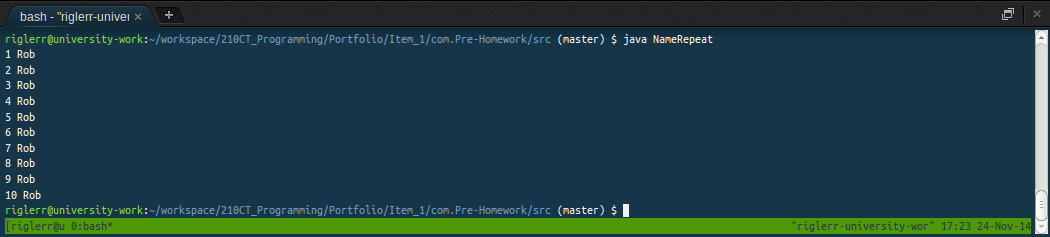
\includegraphics[width=1.0\columnwidth, height=130px]{Item_1/NameRepEvi.png}
\end{center}
}
\clearpage
\homeworkSection{Pre-Homework 2: Write a function that draws a square of stars given as a parameter}
\Cscript{Item_1/com.Pre-Homework/src/StarSquare}{ StarSquare class JAVA code}
\problemAnswer{
\begin{center}\textbf{\underline{Evidence}}

\hspace{10mm}
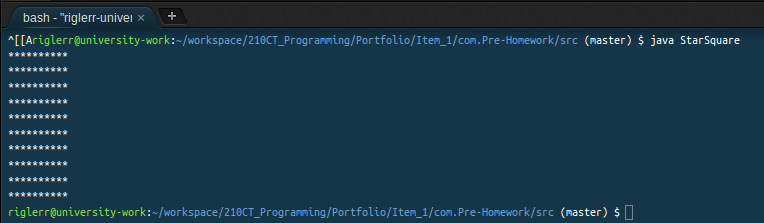
\includegraphics[width=1.0\columnwidth, height=130px]{Item_1/StarSqEvi.png}
\end{center}
}
\clearpage
\homeworkSection{Pre-Homework 3: Write a program to open a file and display it's contents in capitals}
\Cscript{Item_1/com.Pre-Homework/src/RtoCaps}{ RtoCaps class JAVA code}
\problemAnswer{
\begin{center}\textbf{\underline{Evidence}}

\hspace{10mm}
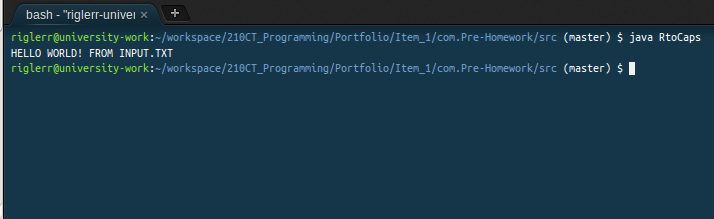
\includegraphics[width=1.0\columnwidth, height=130px]{Item_1/RtcEvi.png}
\end{center}
}

\homeworkSection{ 1. Pseudocode for linear search}

\begin{algorithm}
\begin{algorithmic}
\caption{LinearSearch}
\Procedure{BOOL LINEARSEARCH}{$item$, $list$[\hspace{1mm}]}
\For {each element $i$ in $list$}
\If{ $list[i] = list$}

\indent \indent	\Return true
\EndIf
\EndFor

\Return false
\EndProcedure
\end{algorithmic}
\end{algorithm}
\end{homeworkProblem}

\homeworkSection{ 2. Pseudocode for finding duplicates in a list}
\begin{algorithm}
\caption{Examining for duplicates}
\begin{algorithmic}
\Procedure{BOOL EXFORDUPES}{$list$[\hspace{1mm}]}
\For { each element $i$ in $list$[\hspace{1mm}]}
\For { each element $j$ in $list$[\hspace{1mm}]}
\If{ $list[i] = list[j]$}

\indent \indent \indent \Return true
\EndIf
\EndFor
\EndFor
\EndProcedure
\end{algorithmic}
\end{algorithm}


%----------------------------------------------------------------------------------------
%	PROBLEM 2
%----------------------------------------------------------------------------------------

\begin{homeworkProblem}[Item 2: Week 4 - Big-O of Linear Search and Duplicate Finder  Additional work]



\end{homeworkProblem}
\clearpage
%----------------------------------------------------------------------------------------
%	PROBLEM 3
%----------------------------------------------------------------------------------------
\begin{homeworkProblem}[Item 3: Week 6 - Harmonic Series or Pivot Selection]{}





\end{homeworkProblem}
\clearpage
%----------------------------------------------------------------------------------------
%	PROBLEM 4
%----------------------------------------------------------------------------------------
\begin{homeworkProblem}[Item 4: Week 7 - Heapworksheet or RPN Calculator]{}

\end{homeworkProblem}
%----------------------------------------------------------------------------------------
%	PROBLEM 5
%----------------------------------------------------------------------------------------
\begin{homeworkProblem}[Item 5: Week 8 - Linked List Delete function or Linked List Sortings]{}


\end{homeworkProblem}



\end{document}
